\documentclass[dvipdfmx]{jarticle}
\pagestyle{empty}
\usepackage{tikz}
\usetikzlibrary{shapes,calc}
\begin{document}
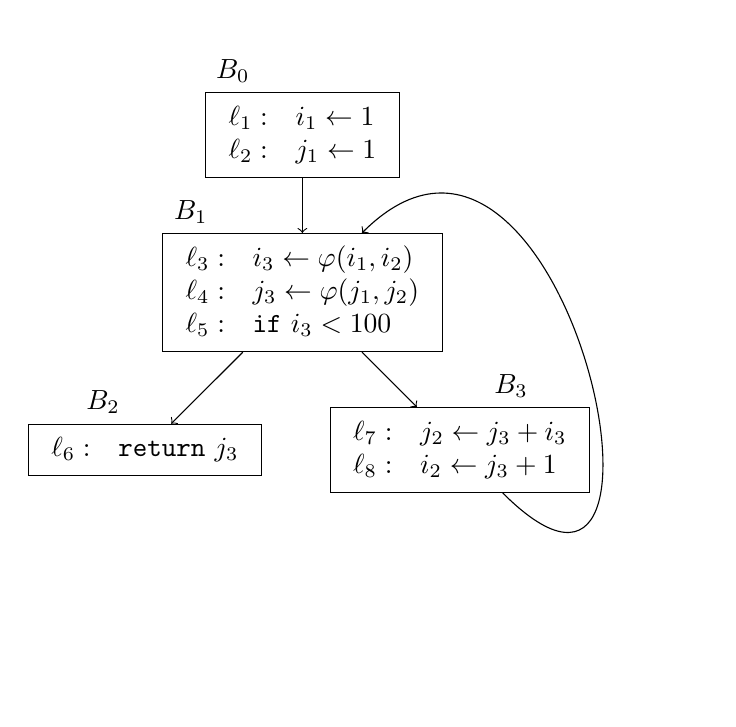
\begin{tikzpicture}
\node[draw,label={135:{$B_0$}}] (N1) at (0,0) {$\begin{array}{ll}
    \ell_1: & i_1\leftarrow 1\\
    \ell_2: & j_1\leftarrow 1\end{array}$};
\node[draw,label={145:{$B_1$}}] (N2) at (0,-2) {$\begin{array}{ll}
    \ell_3: & i_3\leftarrow\varphi(i_1,i_2)\\
    \ell_4: & j_3\leftarrow\varphi(j_1,j_2)\\
    \ell_5: & \texttt{if}\ i_3<100
\end{array}$};
\node[draw,label={120:{$B_2$}}] (N3) at (-2,-4) {$\begin{array}{ll}
    \ell_6: & \texttt{return}\ j_3
\end{array}$};
\node[draw,label={60:{$B_3$}}] (N4) at (2,-4) {$\begin{array}{ll}
    \ell_7: & j_2\leftarrow j_3+i_3\\
    \ell_8: & i_2\leftarrow j_3+1
\end{array}$};
\path[->] (N1) edge (N2) (N2) edge (N3) (N2) edge (N4);
\path[->] (N4) edge [out=315,in=45,looseness=2.5] (N2);
\end{tikzpicture}
\end{document}